%!TEX Root = ./main.tex
\section{Usage Guide}
This section will provide a brief overview of how to use the current package.
The PHASOR package can be downloaded at present from \texttt{https://github.com/ipcamit/phasor} repository, and is available under \textit{GNU GPL v3.0} license.
After downloading/cloning the working directory, open MATLAB and go to the directory containing all functions (named \textit{`phasor/functions'}).
To start, type \texttt{temdatagui} in MATLAB.
You shall see the the GUI window shown in Figure \ref{fig:temdatagui}
\begin{figure}
    \centering
    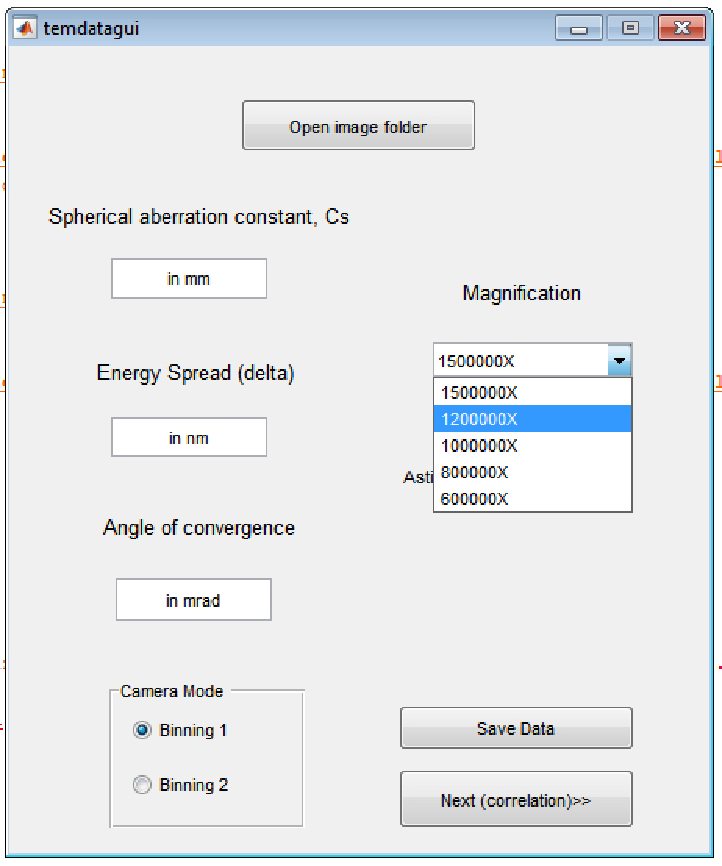
\includegraphics[width=0.6\textwidth]{figures/temdatagui.pdf}
    \caption{GUI window for acquiring initial parameters}
    \label{fig:temdatagui}
\end{figure}

Here all required data fields are to be filled, binning 2 mode is provided as a shortcut to reduce all calibration by a factor of two, as binning two images sometimes provides better signal to noise ratio.
All magnification values are calibrated for JEOL JEM 2100F at Chemical Sciences Devision, IISc, to customize it, provide own calibration value for each magnification in \texttt{switch} statement in \texttt{temdatagui.m} file at line 70.

Once all fields are filled, click on \textit{Open image folder} button, and select the folder containing all the images.
All images shall be present in serial order.

To save the provided data for next time, click on \textit{Save data}/
Then for image alignment click on \textit{Next(correlation)}

\begin{figure}
    \centering
    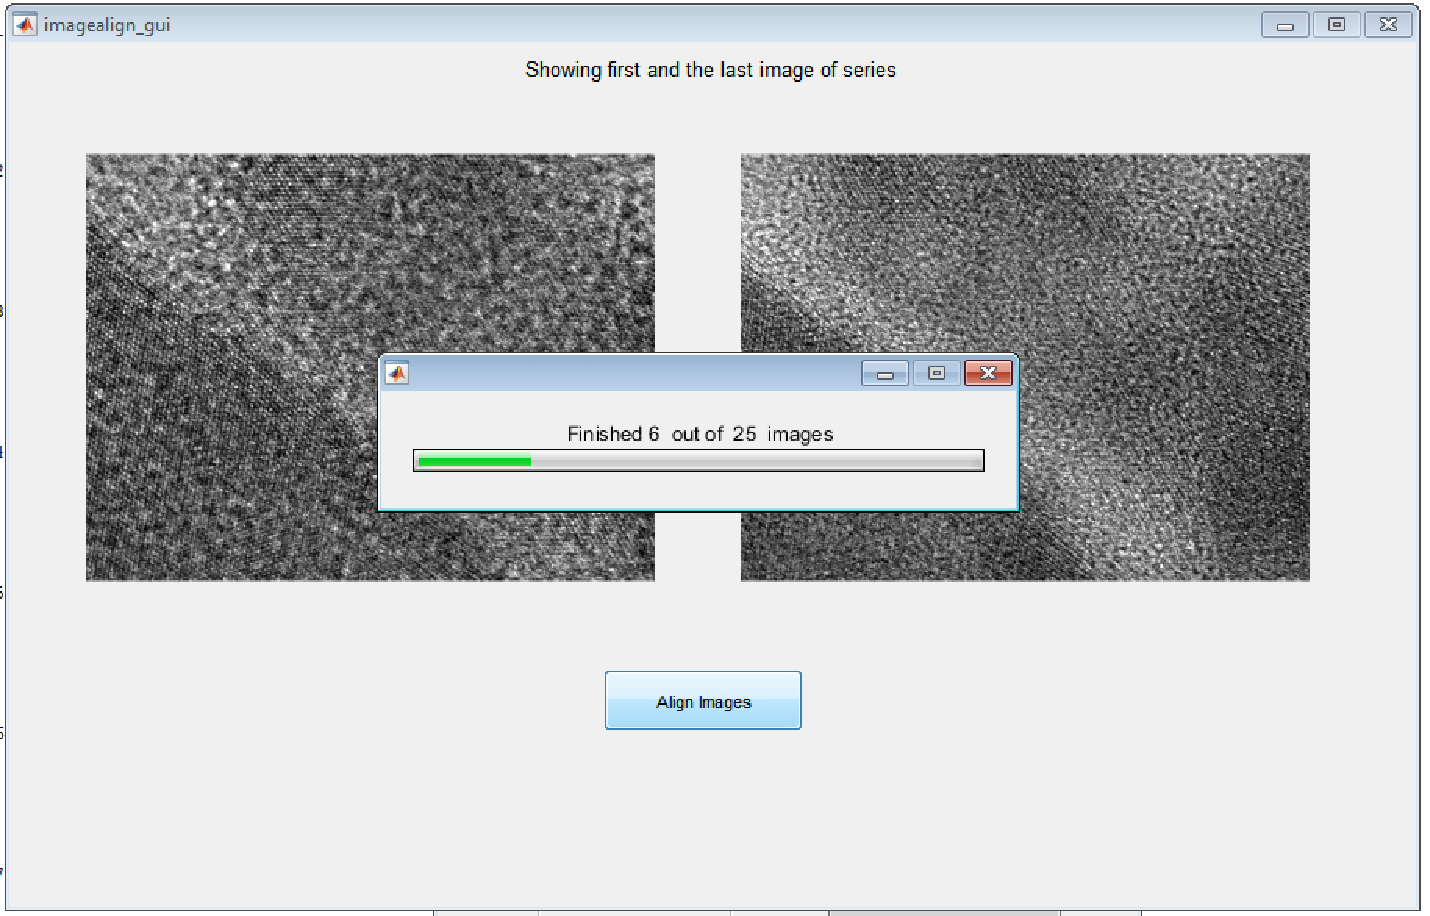
\includegraphics[width=0.6\textwidth]{figures/imalign.pdf}
    \caption{GUI window for aligning images}
    \label{fig:imalign}
\end{figure}

This shall open GUI for aligning images with display containing first and last image in the series.
Once `Align images' is clicked it shall ask the approximate defocus between 2 images (same can be achieved manually by \texttt{imgalign\_gui.m}).
Images are then propagated to that defocus value for better correlation estimation.\cite{meyer_symmetric}
After aligning images it will calculate FFT (using \texttt{fft\_profiler.m} file) for each image and shall present the GUI for defocus estimation.

\begin{figure}
    \centering
    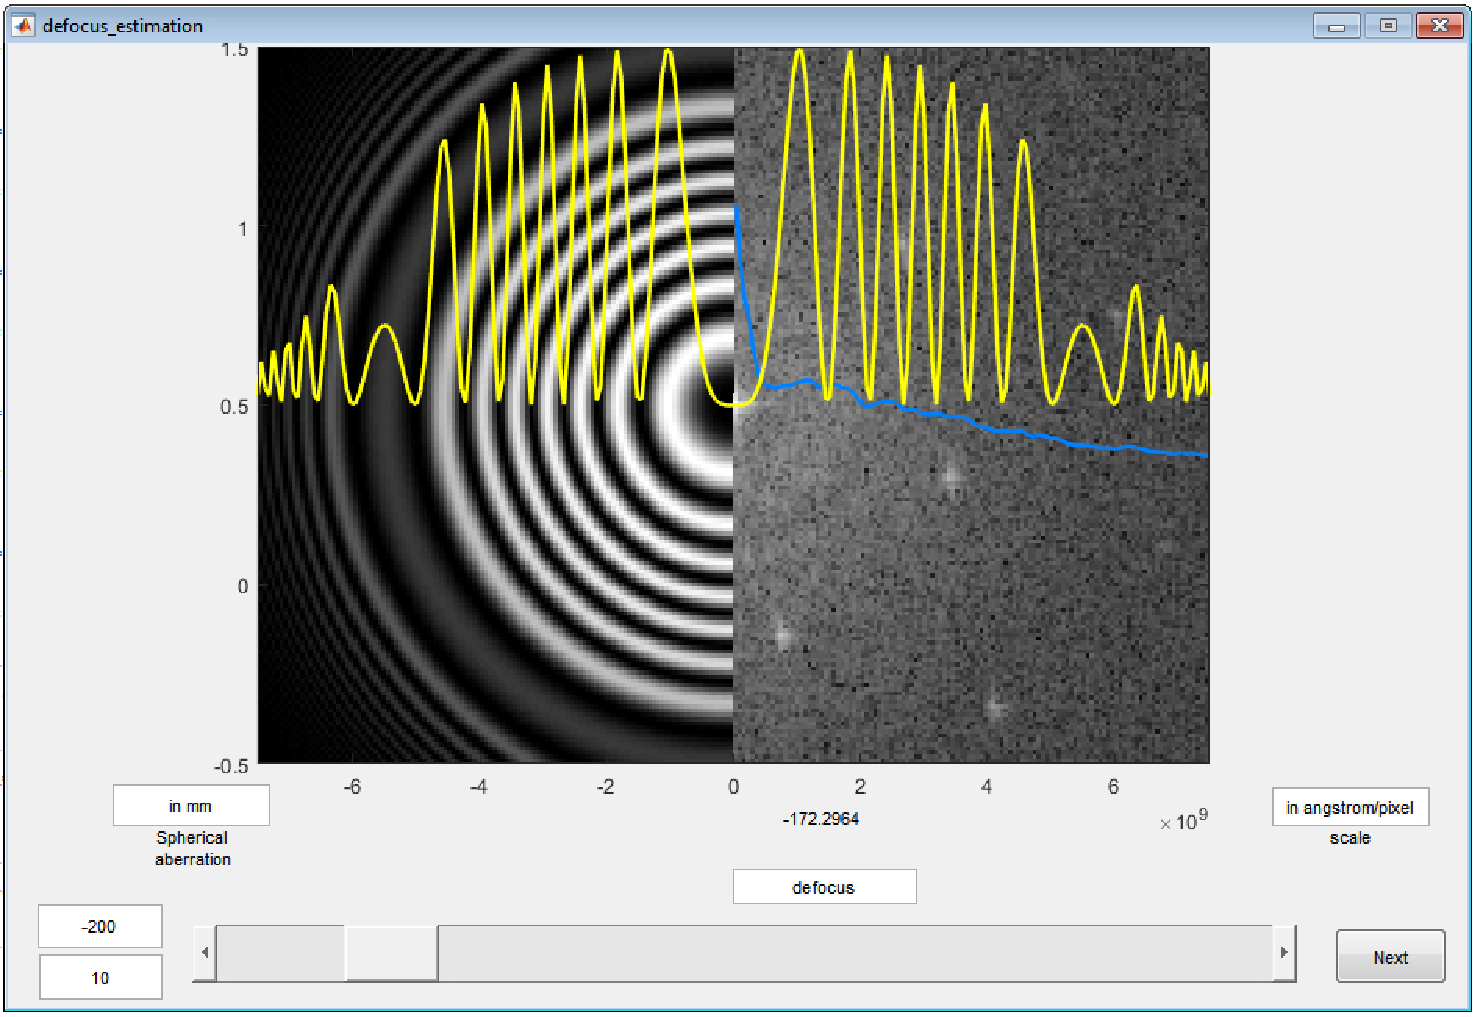
\includegraphics[width=0.6\textwidth]{figures/defocusgui.pdf}
    \caption{GUI window for estimating defocus}
    \label{fig:defocusest}
\end{figure}

Defocus estimation GUI (can also be launched manually by \texttt{defocus\_estimation.m}) will provide two input boxes on left bottom to give custom defocus range.
This serve as a smooth/coarse setting for slider as well.
You can edit lower bound and upper bound for the defocus slider and slider will accordingly adjust its values.
Current defocus value is displayed below the display window (-172.29 nm in current snapshot).
To go to any specific defocus value, enter the defocus value in defocus input box in the middle.
Spherical aberration and magnification can be changes here as well for better fit, but should be avoided.

Once defocus is estimated by matching minima of simulated CTF function (yellow curve) to the minima of acquired data (blue curve), press next to move to next image in series.
Once all images are done you shall be provided with calculated phase and amplitude.
All these results shall be saved in a \textit{'../usr\_data} folder as \texttt{*.mat} file which can be loaded later on for further processing if required.

Limitation: Modulus transfer function has to be calculated by \texttt{MTFestimate.p} program, which due to licensing agreement, cannot be included in current codes.\cite{VandenBroek2012}
Hence user has to obtain it on own and generate MTF file, name it as \texttt{MTF\_2d.mat} and keep it in \textit{../common\_data} folder.
This file is required by \texttt{gen\_mtf.m} function.
